\documentclass{scrartcl}
\usepackage{amsmath,amssymb,graphicx,wrapfig}
\setkomafont{disposition}{\normalfont\bfseries}

\title{Foundations of Computer Science}
\subtitle{Notes from 02-26-2015}
\author{Kenny Roffo}

\begin{document}

\maketitle
\tableofcontents

\section{Formal Languages}

\subsection{Definitions}

\begin{enumerate}

\item A \underline{symbol} is the basic indivisible entity

Natural Languages: words, not letters

\item An \underline{alphabet} is a finite, nonempty set of symbols

$\Sigma$ is typically used as the name for the alphabet

Natural languages: $\Sigma=\{$\emph{all words in English}$\}$ - Lexicon 

\item A \underline{string} (over $\Sigma$) is a finite sequence of symbols (over $\Sigma$)

  Properties: \begin{itemize}
  \item \underline{length}
  \item \underline{empty string} denoted $\lambda$
  \item \underline{concatenation}
  \item $\lambda$ identity of concatenation
  \end{itemize} 

\item $\Sigma ^*$ is the set of all finite strings over $\Sigma$

e.q. $\Sigma=\{0,1\}$, $\Sigma ^* = \{$all strings of $0$ and $1\}$

$\Sigma$ is an alphabet\\
$\Sigma ^*$ is defined recursively

$\lambda$ is an element of $\Sigma ^*$, and if $w \in \Sigma ^*, a \in \Sigma$, then $wa \in \Sigma ^*$

\item A \underline{language} $L$ is any set of strings formed from a given alphabet $\Sigma$\\
$\phi$ is a language over \emph{any} alphabet\\
$\Sigma$ is a language over $\Sigma$\\
$\Sigma ^*$ is a language over $\Sigma$
\end{enumerate}

\subsection{Examples}

\begin{enumerate}

\item $\Sigma = \{b\}$\\
$\Sigma^*=\{\lambda, b, bb, bbb, ...\}$

\item $\Sigma = \{a,b\}$\\
$\Sigma^*=\{\lambda, a, b, aa, ab, ba, bb, ...\}$\\
L is a language over $\Sigma$ that is defined recursively:
ex: $L=\{w|w=a^nb^n, n\ge1\}$\\
($a^n$ means $aaa...a$ n times)\\
Thus $L=\{ab, aabb, aaabbb, aaaabbbb, ...\}$, if $w \in L$, then $awb \in L$\\\\

\item Let $L_n={a^nb^n}$. Then $L = L_0 \cup L_1 \cup L_2 \cup ... $

\item Let $\Sigma_i$ be the language of $i$ length strings in the alphabet $\Sigma=\{a,b\}$.\\
Then $\Sigma_0=\{\lambda\}$, $\Sigma_1=\{a,b\}$, $\Sigma_2=\{aa, ab, ba, bb\}$, ...\\
It follows that the language $\Sigma^*=\Sigma_0 \cup \Sigma_1 \cup \Sigma_2 \cup ...=\bigcup_{i=1}^{\infty} \Sigma_i$

\end{enumerate}

\subsection{What is $\Sigma^*$}

Concatenation - Making new strings from existing strings. We can also concatenate strings with languages and languages with languages.
If $L_1$ and $L_2$ are languages, then $L_1L_2=\{w_1w_2|w_1 \in L_1, w_2 \in L_2\}$\\

ex: Let $L_1=\{$in,out$\}$ and $L_2=\{$law,door,ward$\}$.

Then $L_1L_2=\{$inlaw,outlaw,indoor,outdoor,inward,outward$\}$\\\\
$\Sigma^*$ is the set of all strings made from the alphabet $\Sigma$. But why $\Sigma^*$?\\
$\Sigma^*$ is the result of concatenating $\Sigma$ with itself zero or more times.\\
$\Sigma^+$ is the result of concatenating $\Sigma$ with itself one or more times.

This is called the positive closure of $\Sigma$.\\\\

\section{Regular Expressions}

\subsection{What is a Regular Expression?}

A \emph{regular expression} (regex) is a way to specify patterns for strings using union (or), concatenation, and $^*$\\\\
A regex over $\Sigma$ is defined:

\emph{Basis}: Every $a \in \Sigma$ is a regex over $\Sigma$

\emph{Recursive}: If $u$ and $v$ are regex over $\Sigma$ then $u|v$, $uv$, and $u^*$ are all regex over $\Sigma$\\\\
Here, $|$ means \emph{or} and $^*$ means 0 or more. When in doubt, use parentheses.\\\\
grep - general regular expression parser - a Unix command which searches a file for a pattern defined by a regex.\\\\
Let $X=\{a,ab,aba\}$ and $Y=\{b,bb\}$. Then
\begin{itemize}
\item $XY=\{ab,abb,abb,abbb,abab,ababb\}$ (Concatenation)
\item $X|Y=\{a,ab,aba,b,bb\}$ (Like union)
\item $X^*=\{a,aa,aaa,...,aab,ab,abab,ababab,...,aab,aaba,aaab,ababa,...\}$ 

(All possible strings from 0 or more concatenations)
\item $ababa \in X^*$
\item $ababa \in XY^*$
\item $ab(ab)^*a$ is a regex that matches $ababa$
\end{itemize}

\section{Finite State Machines}
\subsection{The Vending Machine}
Consider a vending machine which contains Jelly beans and Gum. The Machine has inputs
\begin{itemize}
\item N - 5 cents
\item D - 10 cents
\item J - Jelly Bean (Costs 20 cents)
\item G - Gum (Costs 15 cents)
\end{itemize}\pagebreak
These can be represented by $\Sigma=\{N,D,J,G\}$. The machine also has outputs
\begin{itemize}
\item b - beep when money is added
\item j - jelly bean dispensed
\item g - gum dispensed
\end{itemize}
Design a \underline{Finite State} machine - a machine with a finite number of ``things to remember''
This vending machine has to ``remember'':
\begin{itemize}
\item total money deposited (but not he order in which coins are desposited)
\item which product is selected
\end{itemize}
States are drawn with circles and named on the inside:\\

\begin{wrapfigure}[15]{r}[12pt]{3in}
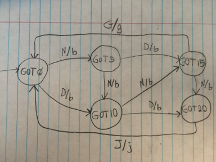
\includegraphics{./VMStateDiagram.png}\\
\end{wrapfigure}

For our Vending Machine the states are described by how much money is in the machine, and the transitions represent money input, or a purchase or gum or a jelly bean. The states live in the set $Q=\{GOT\emptyset,GOT5,GOT10,GOT15,GOT20\}$. State transitions are defined by a function $\delta: Q\times\Sigma\rightarrow Q$. As an example, 
\begin{displaymath}
(GOT5)(N) \rightarrow GOT10 
\end{displaymath}

\end{document}
